\begin{center}
    \Huge{\textbf{\underline{Exercise 1}}}
\end{center}

\vspace{0.45cm}

\textbf{\underline{Solution\(_1\)}}\\[0.1cm]
\begin{center}
    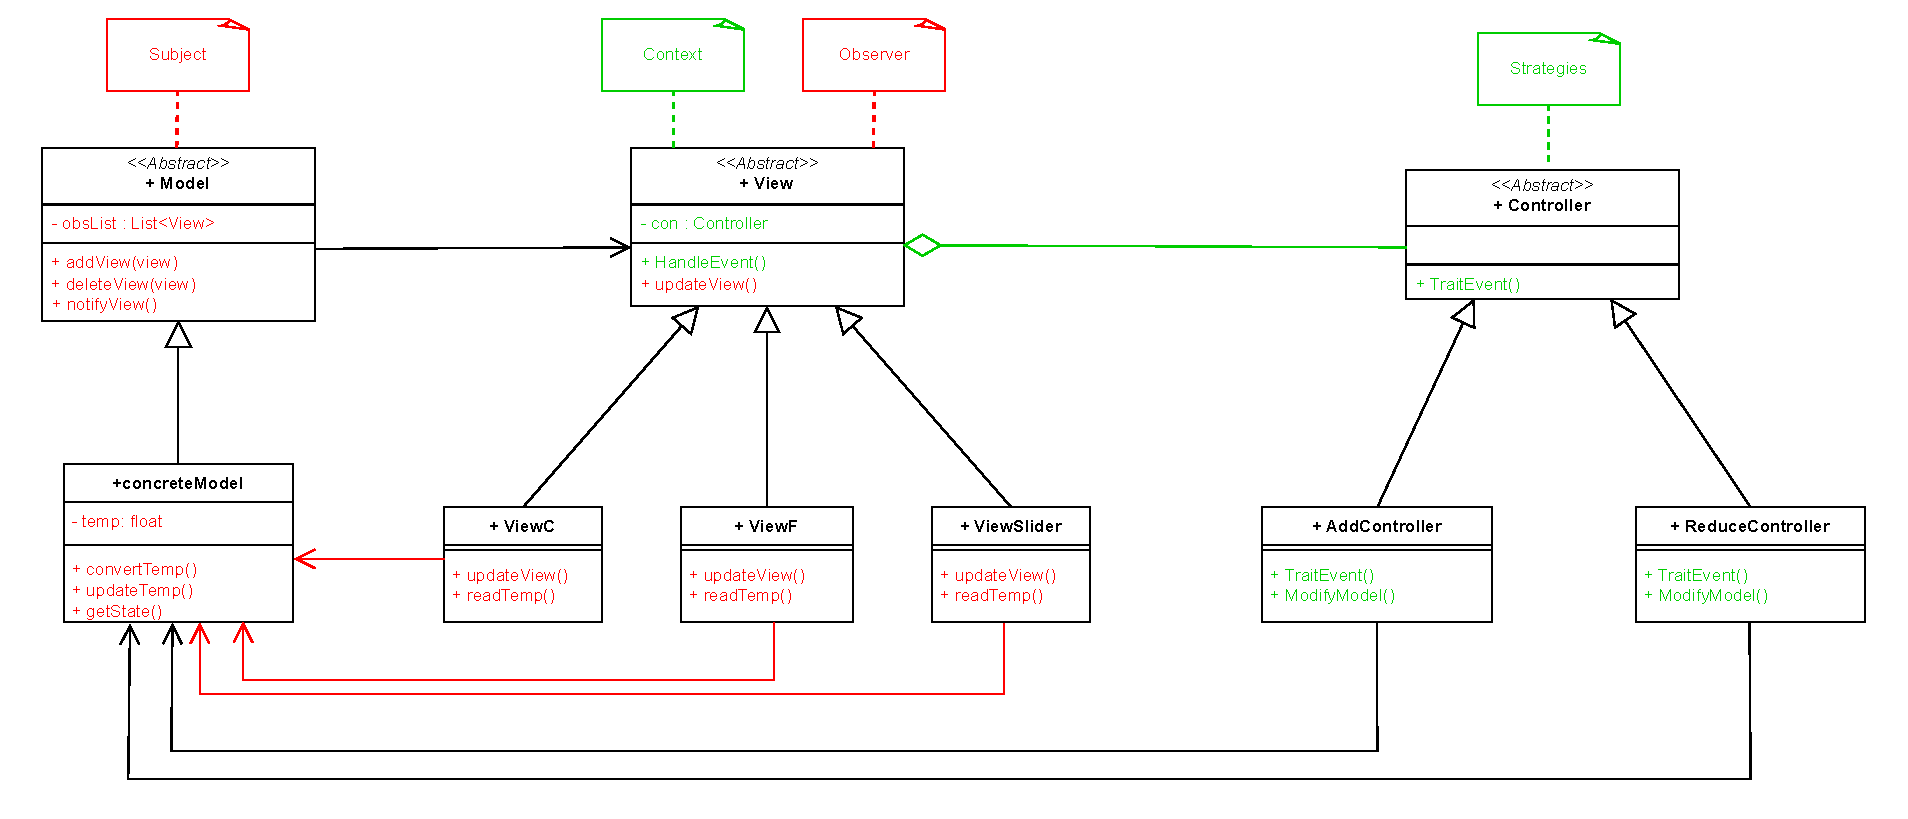
\includegraphics[height=0.22\textheight]{Exercices/EX1/ex1.1.drawio.pdf}
\end{center}

\vspace{0.25cm}

\begin{prettyBox}{Explication}{myblue}
\begin{itemize}
    \item \textbf{The View}: we have 3 views in this app:
        \begin{itemize}
            \item \texttt{ViewC}: displays the temperature in Celsius with - and + buttons.
            \item \texttt{ViewF}: displays the temperature in Fahrenheit with - and + buttons.
            \item \texttt{ViewSlider}: displays the temperature with a slider.
        \end{itemize}
        \texttt{readTemp()}: calls the \texttt{getState()} method of the \texttt{concreteModel}.  
        When the user triggers an event, the \texttt{HandleEvent()} method is called, which in turn calls the \texttt{TraitEvent()} method of the controller class.

    \item \textbf{Controller}: we have 2 types of events, either increasing or decreasing the temperature. Therefore, we have 
        2 subclasses: \texttt{AddController} and \texttt{ReduceController}.  
        \texttt{TraitEvent()} calls \texttt{ModifyModel()}, which then calls the \texttt{updateTemp()} method of \texttt{concreteModel}.

    \item \textbf{Model}: after the temperature is updated, the \texttt{notifyView()} method loops through all views in the list 
        and calls their \texttt{updateView()} method.
\end{itemize}
\end{prettyBox}

\newpage
\textbf{\underline{Solution\(_2\)}}\\[0.1cm]
\begin{center}
    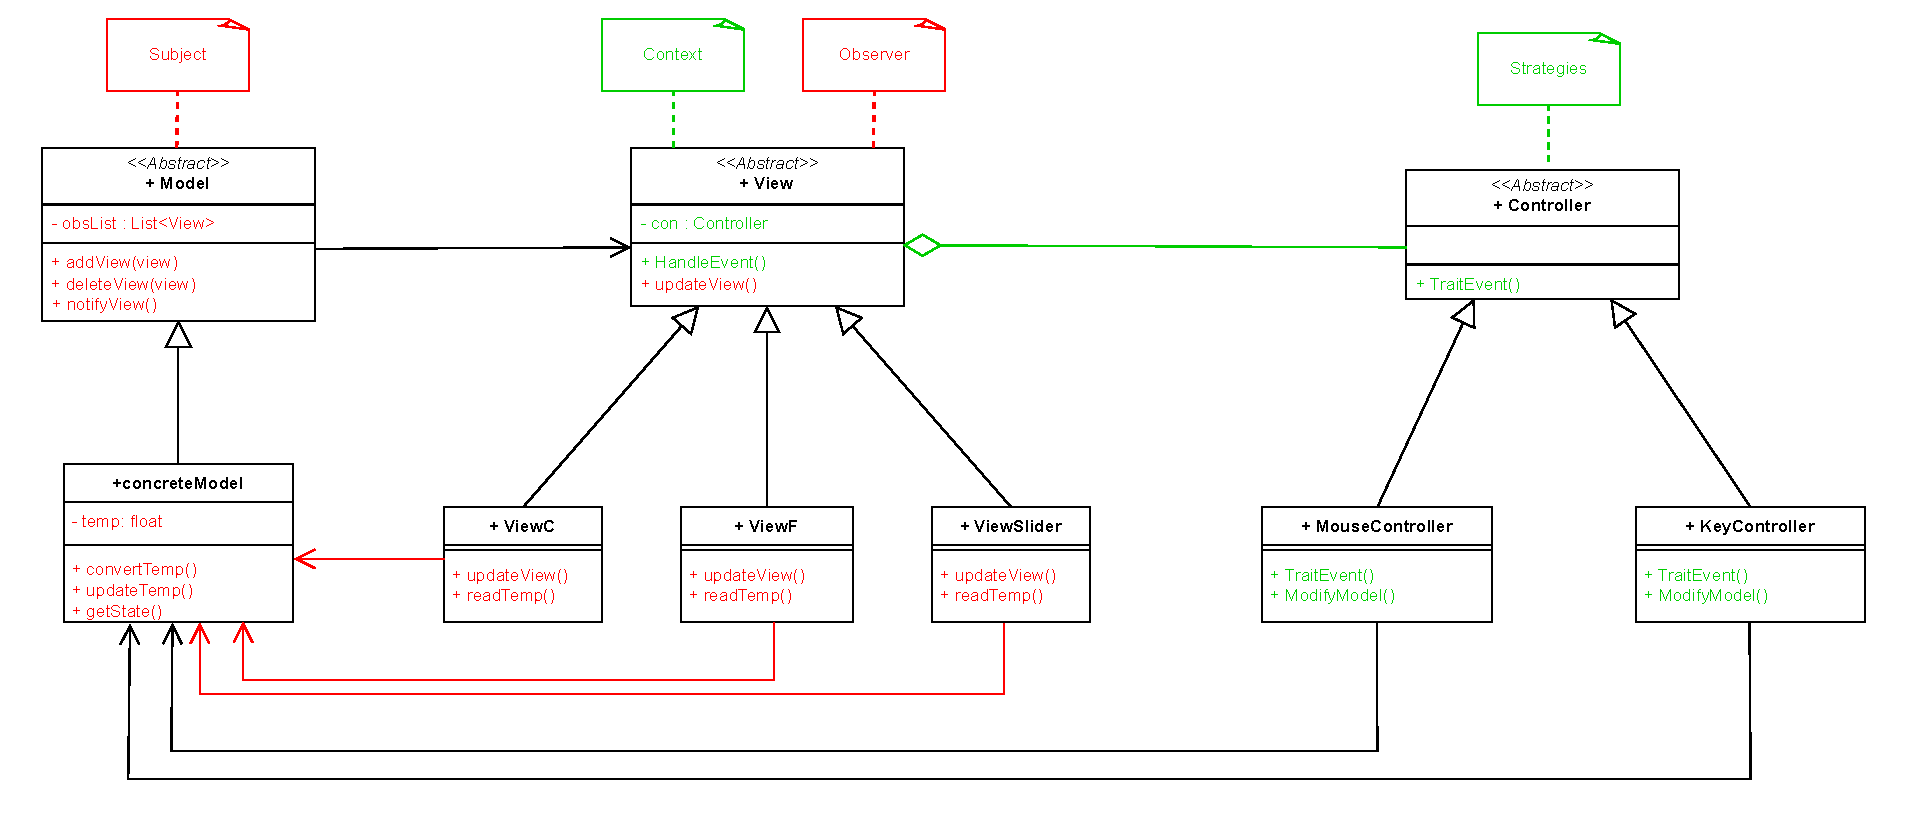
\includegraphics[height=0.22\textheight]{Exercices/EX1/ex1.2.drawio.pdf}
\end{center}


\vspace{0.25cm}

\begin{prettyBox}{Note}{red}
This solution is very similar to the first one. The only difference is that, instead of having two events 
for increasing and decreasing the temperature, we now have keyboard and mouse events. \\[0.15cm]
In theory, this should work, but in some tools and languages, it might cause issues if the slider 
cannot be used with keyboard arrow keys. This would mean that the \textbf{strategies aren't interchangeable} , violating
the \textbf{Strategy} Design Pattern
\end{prettyBox}

